\documentclass[tikz,border=6pt]{standalone}
\usepackage[T1]{fontenc}
\usepackage{lmodern}
\usepackage[utf8]{inputenc}
\usepackage{pgfplots}
\usepgfplotslibrary{groupplots}
\usetikzlibrary{calc}
\pgfplotsset{compat=1.18}
\begin{document}
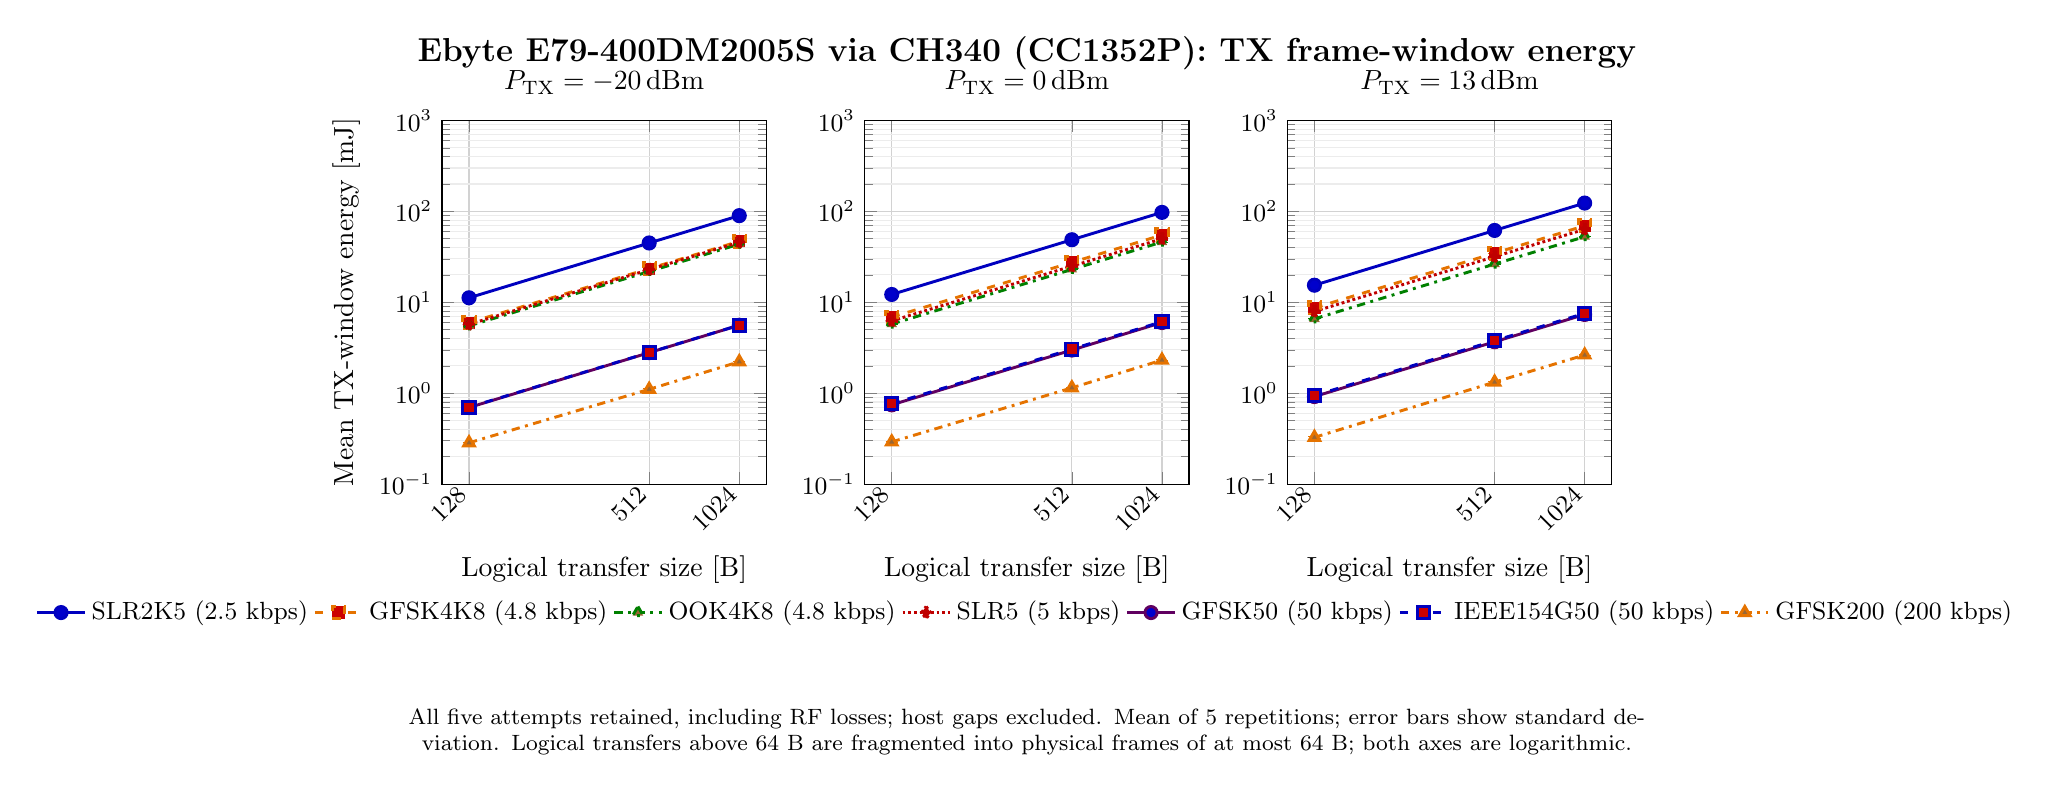
\begin{tikzpicture}
\begin{groupplot}[/pgf/number format/use comma,
  group style={group size=3 by 1, horizontal sep=1.25cm},
  width=5.7cm, height=6.2cm,
  xmode=log, log basis x={2}, ymode=log, log basis y={10},
  ymin=0.1, ymax=1000,
  xtick={128,512,1024}, xticklabels={128,512,1024},
  x tick label style={rotate=45, anchor=east, font=\small},
  y tick label style={font=\small},
  grid=both, minor grid style={gray!15}, major grid style={gray!35},
  xlabel={Logical transfer size [B]},
  every axis plot/.append style={line width=1.05pt},
  error bars/error bar style={line width=0.35pt},
  legend style={font=\small, draw=none, fill=none, at={(0.5,-0.29)},
    anchor=north, legend columns=-1},
]
\nextgroupplot[title={\(P_{\mathrm{TX}}=-20\,\mathrm{dBm}\)}, ylabel={Mean TX-window energy [mJ]}]
\addplot+[
  color=blue!75!black, solid, mark=*, mark size=2.2pt,
  error bars/.cd, y dir=both, y explicit,
] coordinates {
  (128,11.1928728) +- (0,0.0557566886)
  (512,44.8774479) +- (0,0.0456524488)
  (1024,89.6275903) +- (0,0.186865584)
};
\addplot+[
  color=orange!90!black, dashed, mark=square*, mark size=2.2pt,
  error bars/.cd, y dir=both, y explicit,
] coordinates {
  (128,5.97030807) +- (0,0.143613585)
  (512,23.4278723) +- (0,0.335157996)
  (1024,46.8188959) +- (0,0.300476601)
};
\addplot+[
  color=green!50!black, dashdotted, mark=triangle*, mark size=2.2pt,
  error bars/.cd, y dir=both, y explicit,
] coordinates {
  (128,5.49953792) +- (0,0.0121029956)
  (512,21.7892332) +- (0,0.0674737777)
  (1024,43.5989029) +- (0,0.104630747)
};
\addplot+[
  color=red!75!black, densely dotted, mark=diamond*, mark size=2.2pt,
  error bars/.cd, y dir=both, y explicit,
] coordinates {
  (128,5.70892845) +- (0,0.0286870298)
  (512,22.8608259) +- (0,0.0530811682)
  (1024,45.680255) +- (0,0.0488090938)
};
\addplot+[
  color=violet!75!black, solid, mark=*, mark size=2.2pt,
  error bars/.cd, y dir=both, y explicit,
] coordinates {
  (128,0.695007538) +- (0,0.00910719999)
  (512,2.78911809) +- (0,0.0206692534)
  (1024,5.58815108) +- (0,0.0191128269)
};
\addplot+[
  color=blue!75!black, dashed, mark=square*, mark size=2.2pt,
  error bars/.cd, y dir=both, y explicit,
] coordinates {
  (128,0.700830449) +- (0,0.00698620527)
  (512,2.80225596) +- (0,0.0150925663)
  (1024,5.59877082) +- (0,0.0217530059)
};
\addplot+[
  color=orange!90!black, dashdotted, mark=triangle*, mark size=2.2pt,
  error bars/.cd, y dir=both, y explicit,
] coordinates {
  (128,0.284470595) +- (0,0.00441067814)
  (512,1.10265636) +- (0,0.0209415525)
  (1024,2.21484791) +- (0,0.00850634839)
};
\nextgroupplot[title={\(P_{\mathrm{TX}}=0\,\mathrm{dBm}\)}]
\addplot+[
  color=blue!75!black, solid, mark=*, mark size=2.2pt,
  error bars/.cd, y dir=both, y explicit,
] coordinates {
  (128,12.1769815) +- (0,0.00512914954)
  (512,48.7029476) +- (0,0.0135790584)
  (1024,97.3978018) +- (0,0.0448611872)
};
\addlegendentry{SLR2K5 (2.5 kbps)}
\addplot+[
  color=orange!90!black, dashed, mark=square*, mark size=2.2pt,
  error bars/.cd, y dir=both, y explicit,
] coordinates {
  (128,6.85304752) +- (0,0.00850706555)
  (512,27.4492162) +- (0,0.0190090453)
  (1024,54.8768913) +- (0,0.0454415299)
};
\addlegendentry{GFSK4K8 (4.8 kbps)}
\addplot+[
  color=green!50!black, dashdotted, mark=triangle*, mark size=2.2pt,
  error bars/.cd, y dir=both, y explicit,
] coordinates {
  (128,5.75529038) +- (0,0.0166833303)
  (512,22.94814) +- (0,0.0587984613)
  (1024,45.9639922) +- (0,0.0360981701)
};
\addlegendentry{OOK4K8 (4.8 kbps)}
\addplot+[
  color=red!75!black, densely dotted, mark=diamond*, mark size=2.2pt,
  error bars/.cd, y dir=both, y explicit,
] coordinates {
  (128,6.23661102) +- (0,0.00723390604)
  (512,24.9527351) +- (0,0.0228831398)
  (1024,49.8920223) +- (0,0.0346144899)
};
\addlegendentry{SLR5 (5 kbps)}
\addplot+[
  color=violet!75!black, solid, mark=*, mark size=2.2pt,
  error bars/.cd, y dir=both, y explicit,
] coordinates {
  (128,0.744001844) +- (0,0.0019449311)
  (512,2.97966281) +- (0,0.00565175255)
  (1024,5.98012384) +- (0,0.0178744905)
};
\addlegendentry{GFSK50 (50 kbps)}
\addplot+[
  color=blue!75!black, dashed, mark=square*, mark size=2.2pt,
  error bars/.cd, y dir=both, y explicit,
] coordinates {
  (128,0.764196579) +- (0,0.00295888957)
  (512,3.0499602) +- (0,0.00721877697)
  (1024,6.11097273) +- (0,0.0115757077)
};
\addlegendentry{IEEE154G50 (50 kbps)}
\addplot+[
  color=orange!90!black, dashdotted, mark=triangle*, mark size=2.2pt,
  error bars/.cd, y dir=both, y explicit,
] coordinates {
  (128,0.290826449) +- (0,0.0037243396)
  (512,1.14462249) +- (0,0.00752572194)
  (1024,2.3109455) +- (0,0.0201602903)
};
\addlegendentry{GFSK200 (200 kbps)}
\nextgroupplot[title={\(P_{\mathrm{TX}}=13\,\mathrm{dBm}\)}]
\addplot+[
  color=blue!75!black, solid, mark=*, mark size=2.2pt,
  error bars/.cd, y dir=both, y explicit,
] coordinates {
  (128,15.3964456) +- (0,0.0134966644)
  (512,61.6359816) +- (0,0.0442332275)
  (1024,123.308838) +- (0,0.0615516749)
};
\addplot+[
  color=orange!90!black, dashed, mark=square*, mark size=2.2pt,
  error bars/.cd, y dir=both, y explicit,
] coordinates {
  (128,8.67168851) +- (0,0.00665530081)
  (512,34.6970258) +- (0,0.030116824)
  (1024,69.3861012) +- (0,0.0207857755)
};
\addplot+[
  color=green!50!black, dashdotted, mark=triangle*, mark size=2.2pt,
  error bars/.cd, y dir=both, y explicit,
] coordinates {
  (128,6.57332176) +- (0,0.0149980322)
  (512,26.2925627) +- (0,0.0175631853)
  (1024,52.6159028) +- (0,0.0472714242)
};
\addplot+[
  color=red!75!black, densely dotted, mark=diamond*, mark size=2.2pt,
  error bars/.cd, y dir=both, y explicit,
] coordinates {
  (128,7.92702881) +- (0,0.00405458637)
  (512,31.7183579) +- (0,0.0113814351)
  (1024,63.4288784) +- (0,0.0156731368)
};
\addplot+[
  color=violet!75!black, solid, mark=*, mark size=2.2pt,
  error bars/.cd, y dir=both, y explicit,
] coordinates {
  (128,0.917008684) +- (0,0.00348845742)
  (512,3.67305768) +- (0,0.00541599694)
  (1024,7.33433628) +- (0,0.0171076361)
};
\addplot+[
  color=blue!75!black, dashed, mark=square*, mark size=2.2pt,
  error bars/.cd, y dir=both, y explicit,
] coordinates {
  (128,0.941391016) +- (0,0.00288585535)
  (512,3.77801308) +- (0,0.00691954719)
  (1024,7.55078652) +- (0,0.0136924835)
};
\addplot+[
  color=orange!90!black, dashdotted, mark=triangle*, mark size=2.2pt,
  error bars/.cd, y dir=both, y explicit,
] coordinates {
  (128,0.3263859) +- (0,0.00592139815)
  (512,1.32212928) +- (0,0.0130440691)
  (1024,2.62977572) +- (0,0.0172637963)
};
\end{groupplot}
\node[font=\bfseries\large] at ($(group c2r1.north)+(0,0.85cm)$)
  {Ebyte E79-400DM2005S via CH340 (CC1352P): TX frame-window energy};
\node[font=\footnotesize, align=center, text width=18.5cm]
  at ($(group c2r1.south)+(0,-3.15cm)$)
  {All five attempts retained, including RF losses; host gaps excluded. Mean of 5 repetitions; error bars show standard deviation. Logical transfers above 64 B are fragmented into physical frames of at most 64 B; both axes are logarithmic.};
\end{tikzpicture}
\end{document}
